\documentclass[11pt,a4paper]{article}

\usepackage[T1]{fontenc}
\usepackage[utf8]{inputenc}
\usepackage{lmodern}
\usepackage[a4paper,margin=22mm,headheight=15pt]{geometry}
\usepackage{microtype}
\usepackage{amsmath,amssymb,mathtools,bm}
\usepackage{booktabs,array,tabularx}
\usepackage{enumitem}
\usepackage{xcolor}
\usepackage{tikz}
\usetikzlibrary{arrows.meta,calc,positioning}
\usepackage[most]{tcolorbox}
\usepackage{fancyhdr}
\usepackage{titlesec}
\usepackage{hyperref}

\definecolor{ink}{HTML}{17324D}
\definecolor{blue}{HTML}{176B87}
\definecolor{teal}{HTML}{2A9D8F}
\definecolor{gold}{HTML}{E9A23B}
\definecolor{red}{HTML}{C84C4C}
\definecolor{softblue}{HTML}{EAF4F8}
\definecolor{softgold}{HTML}{FFF6E6}
\definecolor{softgreen}{HTML}{EAF7F3}

\hypersetup{
  colorlinks=true,
  linkcolor=blue,
  urlcolor=blue,
  pdftitle={Vectors in Polar Coordinates: A Slow Mechanics Tutorial},
  pdfauthor={Typeset tutorial from handwritten mechanics notes}
}

\pagestyle{fancy}
\fancyhf{}
\fancyhead[L]{\small\color{ink}Vectors in polar coordinates}
\fancyhead[R]{\small\color{blue}A slow mechanics tutorial}
\fancyfoot[C]{\small\color{ink}\thepage}
\renewcommand{\headrulewidth}{0.4pt}
\renewcommand{\headrule}{\hbox to\headwidth{\color{blue}\leaders\hrule height \headrulewidth\hfill}}

\titleformat{\section}{\Large\bfseries\color{ink}}{\color{blue}\thesection}{0.7em}{}
\titleformat{\subsection}{\large\bfseries\color{ink}}{\color{teal}\thesubsection}{0.7em}{}
\titlespacing*{\section}{0pt}{1.2em}{0.6em}
\titlespacing*{\subsection}{0pt}{1em}{0.4em}

\setlength{\parindent}{0pt}
\setlength{\parskip}{0.55em}
\setlist[itemize]{leftmargin=1.5em,itemsep=0.3em,topsep=0.3em}
\setlist[enumerate]{leftmargin=1.7em,itemsep=0.4em,topsep=0.3em}

\newcommand{\er}{\bm e_r}
\newcommand{\etheta}{\bm e_\theta}
\newcommand{\ii}{\bm i}
\newcommand{\jj}{\bm j}
\newcommand{\rr}{\bm r}
\newcommand{\vv}{\bm v}
\newcommand{\acc}{\bm a}
\newcommand{\FF}{\bm F}
\newcommand{\dd}{\mathop{}\!\mathrm d}

\newtcolorbox{idea}[1][]{
  enhanced,breakable,colback=softblue,colframe=blue,
  boxrule=0.7pt,arc=2mm,left=3mm,right=3mm,top=2mm,bottom=2mm,
  title={#1},fonttitle=\bfseries,coltitle=ink
}
\newtcolorbox{notecheck}[1][]{
  enhanced,breakable,colback=softgold,colframe=gold,
  boxrule=0.7pt,arc=2mm,left=3mm,right=3mm,top=2mm,bottom=2mm,
  title={#1},fonttitle=\bfseries,coltitle=ink
}
\newtcolorbox{result}[1][]{
  enhanced,breakable,colback=softgreen,colframe=teal,
  boxrule=0.9pt,arc=2mm,left=3mm,right=3mm,top=2mm,bottom=2mm,
  title={#1},fonttitle=\bfseries,coltitle=ink
}

\begin{document}

\begin{titlepage}
\thispagestyle{empty}
\vspace*{12mm}
{\color{blue}\rule{\textwidth}{1.2pt}}

\vspace{10mm}
{\Huge\bfseries\color{ink}Vectors in Polar Coordinates\par}
\vspace{4mm}
{\LARGE\color{blue}A very slow mechanics tutorial\par}
\vspace{6mm}
{\large\color{ink}From tiny displacements to circular orbits and the law $P\propto r^{3/2}$\par}

\vspace{15mm}
\begin{center}
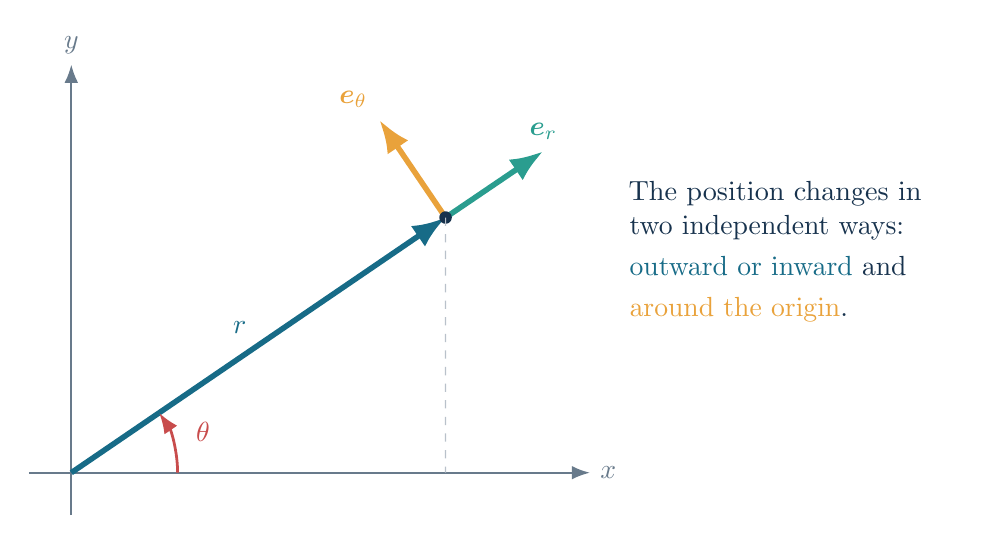
\begin{tikzpicture}[scale=1.08,>=Latex]
  \draw[->,ink!65,line width=0.8pt] (-0.5,0) -- (6.1,0) node[right] {$x$};
  \draw[->,ink!65,line width=0.8pt] (0,-0.5) -- (0,4.8) node[above] {$y$};
  \coordinate (O) at (0,0);
  \coordinate (P) at (4.4,3.0);
  \draw[->,blue,line width=2pt] (O) -- (P) node[midway,above left] {$r$};
  \draw[->,teal,line width=2pt] (P) -- ++(1.15,0.78) node[above] {$\er$};
  \draw[->,gold,line width=2pt] (P) -- ++(-0.78,1.15) node[above left] {$\etheta$};
  \fill[ink] (P) circle (2.1pt);
  \draw[red,line width=1pt,->] (1.25,0) arc[start angle=0,end angle=34.3,radius=1.25];
  \node[red] at (1.55,0.48) {$\theta$};
  \draw[ink!30,dashed] (P) -- (4.4,0);
  \node[anchor=west,text width=4.2cm,align=left,color=ink] at (6.45,2.6)
  {The position changes in two independent ways:\\[1mm]
   \textcolor{blue}{outward or inward} and\\[1mm]
   \textcolor{gold}{around the origin}.};
\end{tikzpicture}
\end{center}

\vfill
\begin{idea}[The single idea to keep in mind]
The Cartesian directions $\ii$ and $\jj$ stay fixed. The polar directions $\er$ and $\etheta$ rotate whenever $\theta$ changes. Most of the apparently new terms in polar acceleration come from differentiating these rotating directions carefully.
\end{idea}

\vspace{8mm}
{\small\color{ink!75}Notation note: $K$ will mean kinetic energy and $P$ will mean orbital period, so the same letter is never asked to do two jobs.\par}
\vspace{7mm}
{\color{blue}\rule{\textwidth}{1.2pt}\par}
\end{titlepage}

\tableofcontents
\thispagestyle{fancy}
\clearpage

\section{What polar coordinates describe}

In a plane, a point can be located by either Cartesian coordinates $(x,y)$ or polar coordinates $(r,\theta)$. The two descriptions refer to the same point:
\[
  x=r\cos\theta,
  \qquad
  y=r\sin\theta.
\]

Here $r\ge 0$ is the distance from the origin and $\theta$ is an angle measured counterclockwise from the positive $x$-axis. In mechanics, both may depend on time:
\[
  r=r(t),
  \qquad
  \theta=\theta(t).
\]

\subsection{The two polar unit vectors}

At the particle we attach two perpendicular unit vectors:

\begin{itemize}
  \item $\er$ points directly away from the origin;
  \item $\etheta$ points in the direction of increasing $\theta$, tangent to the circle $r=\text{constant}$.
\end{itemize}

\subsection{Deriving the unit vectors from little triangles}

The component formulas do not need to be memorised. Draw a short displacement, complete a right triangle, and read off its horizontal and vertical sides.

\begin{center}
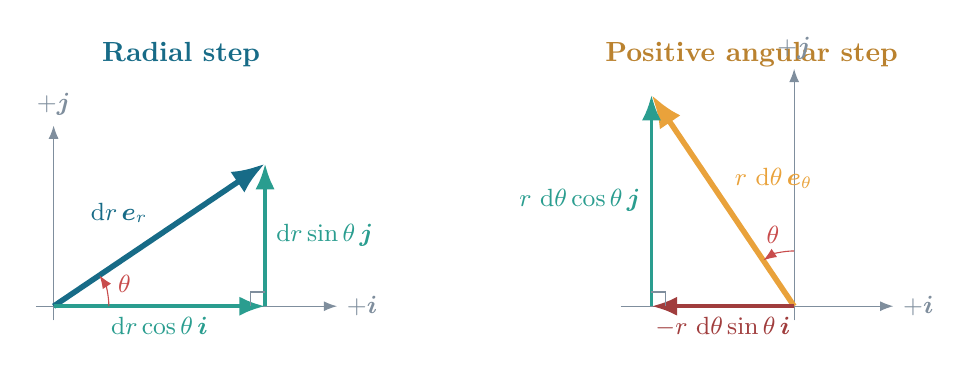
\begin{tikzpicture}[scale=0.90,>=Latex,font=\small]
  % Radial component triangle
  \begin{scope}[xshift=-4.1cm]
    \node[font=\bfseries,color=blue] at (1.8,3.55) {Radial step};
    \coordinate (O) at (0,0);
    \coordinate (P) at ({3.6*cos(34)},{3.6*sin(34)});
    \coordinate (Q) at ({3.6*cos(34)},0);
    \draw[->,ink!55] (-0.25,0) -- (4.0,0) node[right] {$+\ii$};
    \draw[->,ink!55] (0,-0.20) -- (0,2.55) node[above] {$+\jj$};
    \draw[->,blue,line width=2pt] (O) -- (P)
      node[midway,above left] {$\dd r\,\er$};
    \draw[->,teal,line width=1.4pt] (O) -- (Q)
      node[midway,below] {$\dd r\cos\theta\,\ii$};
    \draw[->,teal,line width=1.4pt] (Q) -- (P)
      node[midway,right] {$\dd r\sin\theta\,\jj$};
    \draw[ink!55] ($(Q)+(-0.20,0)$) -- ($(Q)+(-0.20,0.20)$) -- ($(Q)+(0,0.20)$);
    \draw[red,->] (0.78,0) arc[start angle=0,end angle=34,radius=0.78];
    \node[red] at (1.00,0.31) {$\theta$};
  \end{scope}

  % Tangential component triangle
  \begin{scope}[xshift=4.2cm]
    \node[font=\bfseries,color=gold!80!black] at (1.55,3.55) {Positive angular step};
    \coordinate (O) at (2.15,0);
    \coordinate (T) at ({2.15-3.6*sin(34)},{3.6*cos(34)});
    \coordinate (Q) at ({2.15-3.6*sin(34)},0);
    \draw[->,ink!55] (-0.30,0) -- (3.55,0) node[right] {$+\ii$};
    \draw[->,ink!55] (2.15,-0.20) -- (2.15,3.35) node[above] {$+\jj$};
    \draw[->,gold,line width=2pt] (O) -- (T)
      node[midway,above right] {$r\,\dd\theta\,\etheta$};
    \draw[->,red!80!black,line width=1.4pt] (O) -- (Q)
      node[midway,below] {$-r\,\dd\theta\sin\theta\,\ii$};
    \draw[->,teal,line width=1.4pt] (Q) -- (T)
      node[midway,left] {$r\,\dd\theta\cos\theta\,\jj$};
    \draw[ink!55] ($(Q)+(0.20,0)$) -- ($(Q)+(0.20,0.20)$) -- ($(Q)+(0,0.20)$);
    \draw[red,->] ($(O)+(0,0.78)$)
      arc[start angle=90,end angle=124,radius=0.78];
    \node[red] at ($(O)+(-0.30,1.00)$) {$\theta$};
  \end{scope}
\end{tikzpicture}
\end{center}

{\color{blue}\bfseries The radial triangle.}
Take a tiny outward step of length $\dd r$ at angle $\theta$. Its horizontal side is $\dd r\cos\theta$ and its vertical side is $\dd r\sin\theta$. Hence
\begin{align*}
  \dd\rr_{\text{radial}}
  &=\dd r\cos\theta\,\ii+\dd r\sin\theta\,\jj\\
  &=\dd r\left(\cos\theta\,\ii+\sin\theta\,\jj\right).
\end{align*}
Dividing by the step length $\dd r$ leaves the radial unit direction:
\[
  \er=\cos\theta\,\ii+\sin\theta\,\jj.
\]

{\color{gold!80!black}\bfseries The tangential triangle.}
Now increase the angle while keeping $r$ fixed. The tiny arc has length $r\,\dd\theta$ and points $90^\circ$ counterclockwise from $\er$. In the first quadrant it points left and up: its horizontal component is negative, with magnitude $r\,\dd\theta\sin\theta$, while its vertical component is positive, with magnitude $r\,\dd\theta\cos\theta$. Therefore
\begin{align*}
  \dd\rr_{\text{angular}}
  &=-r\,\dd\theta\sin\theta\,\ii
    +r\,\dd\theta\cos\theta\,\jj\\
  &=r\,\dd\theta
    \left(-\sin\theta\,\ii+\cos\theta\,\jj\right).
\end{align*}
Dividing by the tangential step length $r\,\dd\theta$ gives the positive angular unit direction:
\[
  \etheta=-\sin\theta\,\ii+\cos\theta\,\jj.
\]

\begin{idea}[Where the minus sign comes from]
For $0<\theta<\pi/2$, the positive tangential direction goes left and up. Left means a negative $\ii$ component; up means a positive $\jj$ component. The same formula continues to work in every quadrant.
\end{idea}

Collecting the two results,
\begin{result}[Polar basis written in the Cartesian basis]
\[
  \boxed{\er=\cos\theta\,\ii+\sin\theta\,\jj},
  \qquad
  \boxed{\etheta=-\sin\theta\,\ii+\cos\theta\,\jj}.
\]
\end{result}

These are unit vectors and they are perpendicular:
\[
  \er\cdot\er=1,
  \qquad
  \etheta\cdot\etheta=1,
  \qquad
  \er\cdot\etheta=0.
\]

\begin{center}
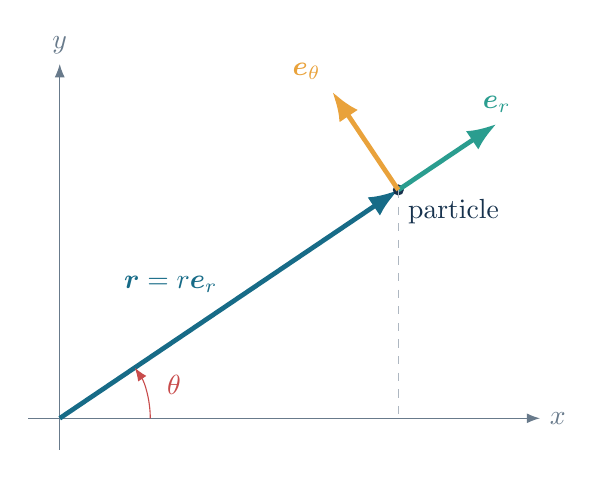
\begin{tikzpicture}[scale=1.0,>=Latex]
  \draw[->,ink!65] (-0.4,0) -- (6.1,0) node[right] {$x$};
  \draw[->,ink!65] (0,-0.4) -- (0,4.5) node[above] {$y$};
  \coordinate (P) at (4.3,2.9);
  \draw[->,blue,line width=1.7pt] (0,0) -- (P) node[midway,above left] {$\rr=r\er$};
  \fill[ink] (P) circle (2pt) node[below right] {particle};
  \draw[->,teal,line width=1.7pt] (P) -- ++(1.25,0.84) node[above] {$\er$};
  \draw[->,gold,line width=1.7pt] (P) -- ++(-0.84,1.25) node[above left] {$\etheta$};
  \draw[red,->] (1.15,0) arc[start angle=0,end angle=34,radius=1.15];
  \node[red] at (1.45,0.43) {$\theta$};
  \draw[ink!35,dashed] (P) -- (4.3,0);
\end{tikzpicture}
\end{center}

\begin{notecheck}[A useful warning]
The symbols $\er$ and $\etheta$ do \emph{not} name two globally fixed directions. Their orientation depends on $\theta$. If the particle moves around the origin, the basis itself turns.
\end{notecheck}

\clearpage

\section{Tiny displacements: one radial, one angular}

Suppose the particle starts at $(r,\theta)$. We first change one coordinate at a time. This separates the geometry before we combine it.

\subsection{Step 1: change $r$, but hold $\theta$ fixed}

Move from $(r,\theta)$ to $(r+\dd r,\theta)$. The motion is along the radial line, so
\[
  \dd\rr_{\text{radial}}=\dd r\,\er.
\]

The scalar $\dd r$ is a signed length. If $\dd r>0$, the displacement is outward; if $\dd r<0$, it is inward.

\subsection{Step 2: change $\theta$, but hold $r$ fixed}

Now move from $(r,\theta)$ to $(r,\theta+\dd\theta)$. The particle follows a tiny circular arc. Its length is
\[
  \text{arc length}=r\,\dd\theta,
\]
provided $\dd\theta$ is measured in radians. The tangent direction is $\etheta$, so
\[
  \dd\rr_{\text{angular}}=r\,\dd\theta\,\etheta.
\]

\begin{center}
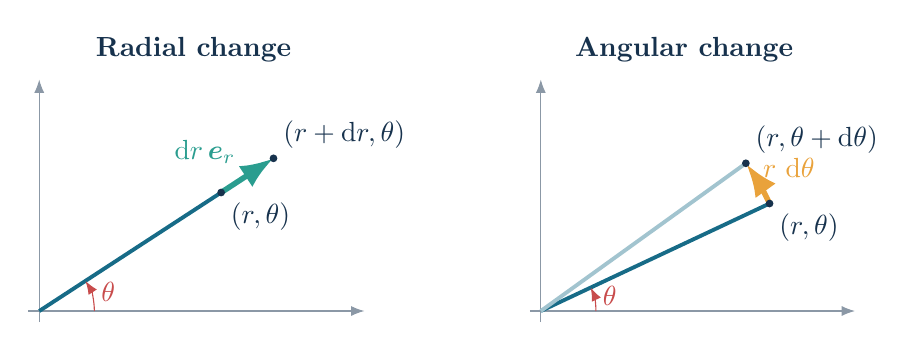
\begin{tikzpicture}[scale=0.70,>=Latex]
  \begin{scope}[xshift=-4.5cm]
    \node[font=\bfseries,color=ink] at (2.8,4.75) {Radial change};
    \draw[->,ink!50] (-0.2,0) -- (5.9,0);
    \draw[->,ink!50] (0,-0.2) -- (0,4.2);
    \coordinate (A) at (3.3,2.15);
    \coordinate (B) at (4.25,2.77);
    \draw[blue,line width=1.4pt] (0,0) -- (A);
    \draw[->,teal,line width=2pt] (A) -- (B) node[midway,above left] {$\dd r\,\er$};
    \fill[ink] (A) circle (2pt) node[below right] {$(r,\theta)$};
    \fill[ink] (B) circle (2pt) node[above right] {$(r+\dd r,\theta)$};
    \draw[red,->] (1.0,0) arc[start angle=0,end angle=33,radius=1.0];
    \node[red] at (1.25,0.34) {$\theta$};
  \end{scope}
  \begin{scope}[xshift=4.6cm]
    \node[font=\bfseries,color=ink] at (2.6,4.75) {Angular change};
    \draw[->,ink!50] (-0.2,0) -- (5.7,0);
    \draw[->,ink!50] (0,-0.2) -- (0,4.2);
    \coordinate (C) at (4.15,1.95);
    \coordinate (D) at (3.72,2.68);
    \draw[blue,line width=1.4pt] (0,0) -- (C);
    \draw[blue!40,line width=1.4pt] (0,0) -- (D);
    \draw[gold,line width=2pt,->] (C) arc[start angle=25.2,end angle=35.7,radius=4.58];
    \fill[ink] (C) circle (2pt) node[below right] {$(r,\theta)$};
    \fill[ink] (D) circle (2pt) node[above right] {$(r,\theta+\dd\theta)$};
    \node[gold] at (4.50,2.60) {$r\,\dd\theta$};
    \draw[red,->] (1.0,0) arc[start angle=0,end angle=25.2,radius=1.0];
    \node[red] at (1.25,0.28) {$\theta$};
  \end{scope}
\end{tikzpicture}
\end{center}

\subsection{Step 3: add the two independent changes}

To first order, a general tiny displacement is the sum:
\begin{result}[Differential displacement in polar coordinates]
\[
  \boxed{\dd\rr=\dd r\,\er+r\,\dd\theta\,\etheta.}
\]
\end{result}

The two coefficients have units of length: $\dd r$ is a length, while $r\dd\theta$ is also a length because an angle in radians is dimensionless.

\begin{notecheck}[Why a tiny change matters]
For a finite angular change, the straight chord and the circular arc are not identical. Their difference enters beyond first order. Differential calculus keeps the terms linear in $\dd r$ and $\dd\theta$, which is exactly what is needed for velocity.
\end{notecheck}

\clearpage

\section{Velocity}

Divide the differential displacement by the elapsed time $\dd t$:
\begin{align*}
  \vv
  =\frac{\dd\rr}{\dd t}
  &=\frac{\dd r}{\dd t}\,\er
    +r\frac{\dd\theta}{\dd t}\,\etheta \\
  &=\dot r\,\er+r\dot\theta\,\etheta.
\end{align*}

\begin{result}[Polar velocity]
\[
  \boxed{\vv=\dot r\,\er+r\dot\theta\,\etheta.}
\]
\end{result}

The two pieces have immediate meanings:

\begin{itemize}
  \item $\dot r\,\er$ is the radial velocity;
  \item $r\dot\theta\,\etheta$ is the tangential velocity.
\end{itemize}

\subsection{A Cartesian cross-check}

Start from
\[
  \rr=x\ii+y\jj,
  \qquad
  x=r\cos\theta,
  \qquad
  y=r\sin\theta.
\]
Differentiate the scalar coordinates:
\begin{align*}
  \dot x&=\dot r\cos\theta-r\dot\theta\sin\theta,\\
  \dot y&=\dot r\sin\theta+r\dot\theta\cos\theta.
\end{align*}
Therefore
\begin{align*}
  \vv
  &=\dot x\ii+\dot y\jj\\
  &=\dot r(\cos\theta\,\ii+\sin\theta\,\jj)
    +r\dot\theta(-\sin\theta\,\ii+\cos\theta\,\jj)\\
  &=\dot r\,\er+r\dot\theta\,\etheta.
\end{align*}

The Cartesian calculation agrees with the geometric one. This is a useful check, but the polar form makes the physical directions much easier to see.

\begin{idea}[Pause and picture it]
If $\dot r=0$, the particle has no inward or outward motion, but it can still be moving: $r\dot\theta$ is its speed around the circle. If $\dot\theta=0$, the direction from the origin is fixed, but the particle may still move radially.
\end{idea}

\clearpage

\section{The basis vectors rotate}

It is tempting to differentiate the velocity as if $\er$ and $\etheta$ were constants. They are not. We now calculate their derivatives explicitly.

\subsection{Differentiate with respect to the angle}

Using their Cartesian expressions,
\begin{align*}
  \frac{\dd\er}{\dd\theta}
  &=\frac{\dd}{\dd\theta}
    (\cos\theta\,\ii+\sin\theta\,\jj)\\
  &=-\sin\theta\,\ii+\cos\theta\,\jj\\
  &=\etheta,
\end{align*}
and
\begin{align*}
  \frac{\dd\etheta}{\dd\theta}
  &=\frac{\dd}{\dd\theta}
    (-\sin\theta\,\ii+\cos\theta\,\jj)\\
  &=-\cos\theta\,\ii-\sin\theta\,\jj\\
  &=-\er.
\end{align*}

\begin{result}[How the polar basis turns]
\[
  \boxed{\frac{\dd\er}{\dd\theta}=\etheta},
  \qquad
  \boxed{\frac{\dd\etheta}{\dd\theta}=-\er}.
\]
\end{result}

The first formula says that a small increase in angle tips $\er$ toward $\etheta$. The second says that the tangent direction bends inward, toward $-\er$.

\subsection{Convert angle derivatives to time derivatives}

Apply the chain rule:
\[
  \frac{\dd\er}{\dd t}
  =\frac{\dd\er}{\dd\theta}\frac{\dd\theta}{\dd t}
  =\dot\theta\,\etheta,
\]
and similarly
\[
  \frac{\dd\etheta}{\dd t}
  =\frac{\dd\etheta}{\dd\theta}\frac{\dd\theta}{\dd t}
  =-\dot\theta\,\er.
\]

\begin{result}[Time derivatives of the rotating basis]
\[
  \boxed{\dot{\er}=\dot\theta\,\etheta},
  \qquad
  \boxed{\dot{\etheta}=-\dot\theta\,\er}.
\]
\end{result}

\clearpage

\section{Acceleration, one product rule at a time}

Begin with the velocity:
\[
  \vv=\dot r\,\er+r\dot\theta\,\etheta.
\]
Differentiate each vector term separately.

\subsection{Step 1: differentiate the radial velocity term}

Use the product rule and $\dot{\er}=\dot\theta\etheta$:
\begin{align*}
  \frac{\dd}{\dd t}(\dot r\,\er)
  &=\ddot r\,\er+\dot r\,\dot{\er}\\
  &=\ddot r\,\er+\dot r\dot\theta\,\etheta.
\end{align*}

\subsection{Step 2: differentiate the tangential velocity term}

The scalar coefficient $r\dot\theta$ and the vector $\etheta$ both vary:
\begin{align*}
  \frac{\dd}{\dd t}(r\dot\theta\,\etheta)
  &=\frac{\dd}{\dd t}(r\dot\theta)\,\etheta
    +r\dot\theta\,\dot{\etheta}\\
  &=(\dot r\dot\theta+r\ddot\theta)\etheta
    +r\dot\theta(-\dot\theta\er)\\
  &=(\dot r\dot\theta+r\ddot\theta)\etheta
    -r\dot\theta^{\,2}\er.
\end{align*}

\subsection{Step 3: collect like directions}

Add the two results. The $\er$ terms go together and the $\etheta$ terms go together:
\begin{align*}
  \acc
  &=\left(\ddot r-r\dot\theta^{\,2}\right)\er
    +\left(\dot r\dot\theta+\dot r\dot\theta+r\ddot\theta\right)\etheta\\
  &=\left(\ddot r-r\dot\theta^{\,2}\right)\er
    +\left(2\dot r\dot\theta+r\ddot\theta\right)\etheta.
\end{align*}

\begin{result}[Polar acceleration]
\[
  \boxed{
  \acc=\left(\ddot r-r\dot\theta^{\,2}\right)\er
  +\left(2\dot r\dot\theta+r\ddot\theta\right)\etheta.}
\]
\end{result}

\begin{notecheck}[The common mistake]
Writing only $\ddot r\er+r\ddot\theta\etheta$ misses the derivatives of the basis vectors. The missing terms, $-r\dot\theta^2\er$ and $2\dot r\dot\theta\etheta$, are not optional corrections; they are required by the geometry.
\end{notecheck}

\clearpage

\section{What the four acceleration terms mean}

The formula is easier to remember when each term has a job:

\begin{center}
\renewcommand{\arraystretch}{1.35}
\begin{tabularx}{\textwidth}{>{\raggedright\arraybackslash}p{31mm} >{\raggedright\arraybackslash}p{31mm} X}
\toprule
\textbf{Term} & \textbf{Direction} & \textbf{Interpretation}\\
\midrule
$\ddot r$ & radial & Change in the radial speed. Positive is outward.\\
$-r\dot\theta^2$ & radial & Inward curvature term. It remains even when the speed around a circle is constant.\\
$r\ddot\theta$ & transverse & Tangential acceleration caused by changing angular speed.\\
$2\dot r\dot\theta$ & transverse & Coupling between radial motion and rotation of the basis, often called the Coriolis term in this coordinate description.\\
\bottomrule
\end{tabularx}
\end{center}

\subsection{A quick dimensional check}

Angles in radians are dimensionless. Therefore
\[
  [\dot r]=LT^{-1},
  \qquad
  [\ddot r]=LT^{-2},
  \qquad
  [\dot\theta]=T^{-1},
  \qquad
  [\ddot\theta]=T^{-2}.
\]
Every coefficient in the acceleration formula has units $LT^{-2}$:
\[
  [r\dot\theta^2]=L(T^{-1})^2=LT^{-2},
\]
\[
  [\dot r\dot\theta]=(LT^{-1})(T^{-1})=LT^{-2},
  \qquad
  [r\ddot\theta]=L(T^{-2})=LT^{-2}.
\]

\begin{idea}[Why the inward term appears at constant speed]
A velocity vector can change even if its magnitude does not. During circular motion the velocity continually turns, so its derivative points toward the centre. The term $-r\dot\theta^2\er$ measures exactly that inward turning.
\end{idea}

\subsection{Three useful special cases}

\begin{enumerate}
  \item \textbf{Pure radial motion:} if $\dot\theta=0$, then $\acc=\ddot r\er$.
  \item \textbf{Motion at fixed radius:} if $r=R$, then
  \[
    \acc=-R\dot\theta^2\er+R\ddot\theta\etheta.
  \]
  \item \textbf{Uniform circular motion:} if $r=R$ and $\dot\theta=\omega$ is constant, then
  \[
    \acc=-R\omega^2\er.
  \]
\end{enumerate}

\clearpage

\section{Speed squared and kinetic energy}

Start again from
\[
  \vv=\dot r\er+r\dot\theta\etheta.
\]
The square of the speed means the dot product $v^2=\vv\cdot\vv$:
\begin{align*}
  v^2
  &=(\dot r\er+r\dot\theta\etheta)
    \cdot(\dot r\er+r\dot\theta\etheta)\\
  &=\dot r^{\,2}(\er\cdot\er)
    +2r\dot r\dot\theta(\er\cdot\etheta)
    +r^2\dot\theta^{\,2}(\etheta\cdot\etheta).
\end{align*}
Now use orthonormality:
\[
  \er\cdot\er=1,
  \qquad
  \er\cdot\etheta=0,
  \qquad
  \etheta\cdot\etheta=1.
\]
The cross term vanishes, leaving
\begin{result}[Speed in polar coordinates]
\[
  \boxed{v^2=\dot r^{\,2}+r^2\dot\theta^{\,2}.}
\]
\end{result}

For a particle of mass $m$, the kinetic energy is
\begin{result}[Kinetic energy in polar coordinates]
\[
  \boxed{K=\frac12m\left(\dot r^{\,2}+r^2\dot\theta^{\,2}\right).}
\]
\end{result}

For circular motion $r=R$ is constant, so $\dot r=0$. If $\dot\theta=\omega$, then
\[
  v=R\omega,
  \qquad
  K=\frac12mR^2\omega^2.
\]

\begin{notecheck}[Dimensions of the energy]
Both $\dot r^2$ and $r^2\dot\theta^2$ have units $L^2T^{-2}$. Multiplication by mass gives $ML^2T^{-2}$, the dimensions of energy.
\end{notecheck}

\clearpage

\section{Uniform circular motion and centripetal force}

The phrase \emph{uniform circular motion} contains several assumptions. We state them before using the shortened formulas.

\begin{itemize}
  \item The radius is constant: $r(t)=R$. Hence $\dot r=0$ and $\ddot r=0$.
  \item The angular speed is constant: $\dot\theta=\omega$. Hence $\ddot\theta=0$.
  \item The only acceleration is radial and inward.
\end{itemize}

Substitute these conditions into the general velocity and acceleration:
\[
  \vv=R\omega\etheta,
  \qquad
  \acc=-R\omega^2\er.
\]
Newton's second law gives
\begin{result}[Force required for uniform circular motion]
\[
  \boxed{\FF=m\acc=-mR\omega^2\er.}
\]
\end{result}

The minus sign says that the force points opposite to $\er$, toward the centre. Its magnitude is
\[
  F_{\text{in}}=mR\omega^2=\frac{mv^2}{R}.
\]

\begin{center}
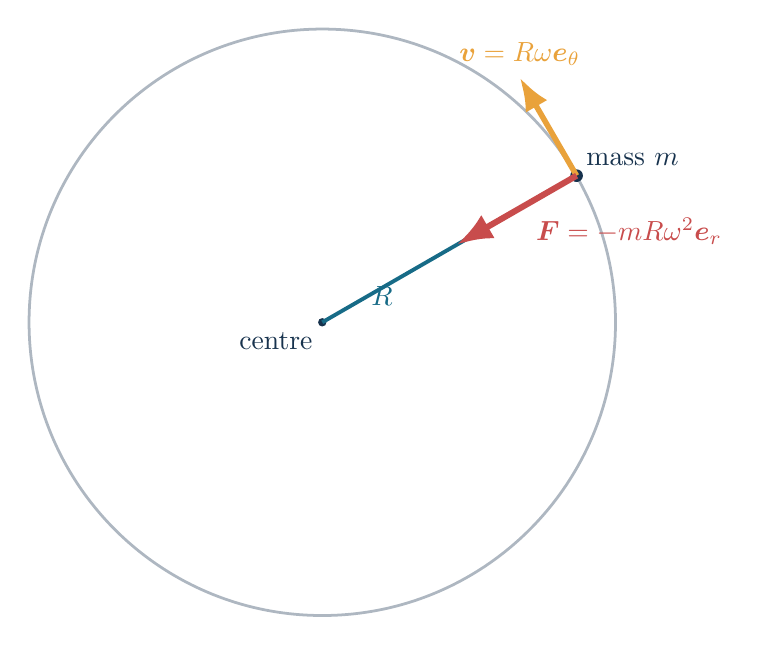
\begin{tikzpicture}[scale=0.76,>=Latex]
  \coordinate (O) at (0,0);
  \coordinate (P) at (4.25,2.45);
  \draw[ink!35,line width=1pt] (O) circle (4.9);
  \fill[ink] (O) circle (2pt) node[below left] {centre};
  \draw[blue,line width=1.4pt] (O) -- (P) node[pos=0.32,below left] {$R$};
  \fill[ink] (P) circle (3pt) node[above right] {mass $m$};
  \draw[->,gold,line width=2pt] (P) -- ++(-0.95,1.64) node[above] {$\vv=R\omega\etheta$};
  \draw[->,red,line width=2.2pt] (P) -- ++(-2.0,-1.15)
    node[pos=0.44,below right] {$\FF=-mR\omega^2\er$};
\end{tikzpicture}
\end{center}

\begin{notecheck}[Circular motion is a special solution]
A central force does not automatically make every orbit circular. A circular orbit requires the correct initial tangential speed and no initial radial speed. Other initial conditions can produce non-circular bound or unbound orbits.
\end{notecheck}

\clearpage

\section{Inverse-square attraction and the orbital period}

We now apply the circular-motion result to an attractive inverse-square field. It is safest to distinguish an \emph{acceleration law} from a \emph{force law}.

\subsection{Form A: inverse-square acceleration}

For gravity around a fixed central mass $M$, define
\[
  \mu=GM.
\]
The gravitational acceleration is
\[
  \acc_{\text{grav}}=-\frac{\mu}{r^2}\er.
\]
For a circular orbit of radius $R$, the required acceleration is $-R\omega^2\er$. Equate their magnitudes:
\begin{align*}
  \frac{\mu}{R^2}&=R\omega^2,\\
  \omega^2&=\frac{\mu}{R^3},\\
  \omega&=\sqrt{\frac{\mu}{R^3}}.
\end{align*}

One revolution is $2\pi$ radians, so the period is
\[
  P=\frac{2\pi}{\omega}.
\]
Substitution gives
\begin{result}[Period of a circular inverse-square orbit]
\[
  \boxed{P=2\pi\sqrt{\frac{R^3}{\mu}}},
  \qquad
  \boxed{P^2=\frac{4\pi^2}{\mu}R^3}.
\]
Therefore, with the same central body fixed,
\[
  \boxed{P\propto R^{3/2}.}
\]
\end{result}

\subsection{Dimensional check}

The gravitational parameter has dimensions
\[
  [\mu]=[GM]=L^3T^{-2}.
\]
Therefore
\[
  \left[\frac{R^3}{\mu}\right]
  =\frac{L^3}{L^3T^{-2}}=T^2,
\]
and its square root has units of time, as a period must.

\clearpage

\subsection{Form B: inverse-square force}

Suppose instead that the force itself is written
\[
  \FF=-\frac{\kappa}{r^2}\er.
\]
Then $\kappa$ must have dimensions $ML^3T^{-2}$. On a circular orbit,
\begin{align*}
  \frac{\kappa}{R^2}&=mR\omega^2,\\
  \omega^2&=\frac{\kappa}{mR^3},\\
  P&=2\pi\sqrt{\frac{mR^3}{\kappa}}.
\end{align*}

For gravity, $\kappa=GMm=\mu m$, so the orbiting mass cancels:
\[
  P=2\pi\sqrt{\frac{mR^3}{GMm}}
   =2\pi\sqrt{\frac{R^3}{GM}}.
\]

\begin{idea}[How this matches shorthand notation]
If a handwritten derivation writes $k/R^2=R\omega^2$, then $k$ is being used as an acceleration parameter with dimensions $L^3T^{-2}$, like $\mu=GM$. If it writes a force $k/R^2$, an additional factor of $m$ belongs in Newton's second law unless $m$ has already been absorbed into $k$.
\end{idea}

\subsection{What has, and has not, been shown}

The calculation above establishes the $R^{3/2}$ scaling for circular orbits in an inverse-square field. Kepler's third law also holds for elliptical two-body orbits when $R$ is replaced by the semi-major axis $a$:
\[
  P^2=\frac{4\pi^2}{\mu}a^3
\]
in the fixed-central-mass approximation. For the full two-body problem, $\mu=G(M+m)$. Those broader results require additional orbital mechanics; the circular derivation here captures the scaling in its simplest setting.

\clearpage

\section{The entire derivation on one page}

\begin{enumerate}
  \item Define the rotating polar basis:
  \[
    \er=\cos\theta\ii+\sin\theta\jj,
    \qquad
    \etheta=-\sin\theta\ii+\cos\theta\jj.
  \]

  \item Resolve a tiny displacement into radial and angular pieces:
  \[
    \dd\rr=\dd r\er+r\dd\theta\etheta.
  \]

  \item Divide by time:
  \[
    \vv=\dot r\er+r\dot\theta\etheta.
  \]

  \item Account for the rotating basis:
  \[
    \dot{\er}=\dot\theta\etheta,
    \qquad
    \dot{\etheta}=-\dot\theta\er.
  \]

  \item Differentiate the velocity:
  \[
    \acc=(\ddot r-r\dot\theta^2)\er
    +(2\dot r\dot\theta+r\ddot\theta)\etheta.
  \]

  \item Use orthonormality to find speed and kinetic energy:
  \[
    v^2=\dot r^2+r^2\dot\theta^2,
    \qquad
    K=\frac12m(\dot r^2+r^2\dot\theta^2).
  \]

  \item For uniform circular motion, set $r=R$ and $\dot\theta=\omega$ constant:
  \[
    \acc=-R\omega^2\er,
    \qquad
    \FF=-mR\omega^2\er.
  \]

  \item Match this to inverse-square gravitational acceleration:
  \[
    \frac{\mu}{R^2}=R\omega^2
    \quad\Longrightarrow\quad
    P=2\pi\sqrt{\frac{R^3}{\mu}}
    \quad\Longrightarrow\quad
    P\propto R^{3/2}.
  \]
\end{enumerate}

\begin{result}[The conceptual thread]
The polar formulas are not mysterious new laws. They are ordinary vector differentiation expressed in a basis that turns with $\theta$. Once the basis derivatives are included, velocity, acceleration, energy, and circular-orbit dynamics follow in a continuous chain.
\end{result}

\vfill
\begin{center}
{\color{blue}\rule{0.55\textwidth}{0.8pt}}\\[2mm]
{\small\color{ink!75}End of tutorial}
\end{center}

\end{document}
